\begin{frame}
    \frametitle{Visualizzare ed Elaborare documenti XML}
    \addtocounter{nframe}{1}
    
    %\begin{center}
    %    
\includegraphics[width=.2\textwidth]{../imgs/tei-r.pdf}
    %\end{center}
    %\textit{In parte già disponibili nei moduli TEI di base}

     \begin{block}{Documenti Object Model (DOM)}
        Il \textbf{Document Object Model} (\textit{DOM}) è un modello \textit{language-independed} che mette a disposizione delle \textbf{Application Programming Interface} (\textit{API}) per accedere e manipolare documenti XML (e HTML).

     \end{block}

     \begin{block}{Documenti Object Model (DOM)}
        Il Modello DOM rappresenta l'intero documento XML come una gerarchia di nodi (\textit{albero}).
     \end{block}


\end{frame}


\begin{frame}
    \frametitle{Visualizzare ed Elaborare documenti XML}
    \addtocounter{nframe}{1}
    \textit{Esempio albero DOM}    
    \begin{center}
        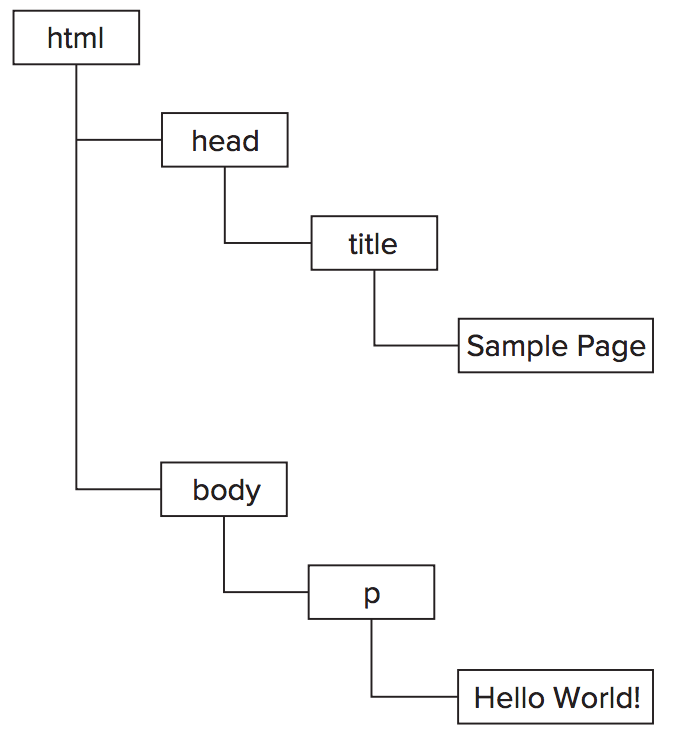
\includegraphics[width=.7\textwidth]{imgs/XML-DOM.png}
    \end{center}


\end{frame}

\begin{frame}
    \frametitle{Visualizzare ed Elaborare documenti XML}
    \addtocounter{nframe}{1}
    
    %\begin{center}
    %    
\includegraphics[width=.2\textwidth]{../imgs/tei-r.pdf}
    %\end{center}
    %\textit{In parte già disponibili nei moduli TEI di base}

     \begin{block}{Documenti Object Model (DOM)}
        Ciascuna parte di un documento XML-TEI è quindi un tipo specifico di nodo DOM costituito da diversi tipi di dati.
     \end{block}

     \begin{block}{Documenti Object Model (DOM)}
        Grazie alla rappresentazione gerarchica messa a disposizione dal DOM è possibile avere un livello di controllo a granularità molto fine per manipolare quasi tutti gli aspetti del documento XML originario.
     \end{block}
     
\end{frame}

\begin{frame}
    \frametitle{Visualizzare ed Elaborare documenti XML}
    \addtocounter{nframe}{1}
    
    %\begin{center}
    %    
\includegraphics[width=.2\textwidth]{../imgs/tei-r.pdf}
    %\end{center}
    %\textit{In parte già disponibili nei moduli TEI di base}

     \begin{block}{Documenti Object Model (DOM): espressività}
        Nodes can be removed, added, replaced, and modified easily by using the DOM API.
     \end{block}

     \begin{block}{Documenti Object Model (DOM)}
        Il modello DOM è una specifica e una raccomandazione del consorzio di standardiziazione Web W3C.
        \\\url{URL/TO/DOM/W3C/RECOMMENDATION}
     \end{block}
     
\end{frame}

\begin{frame}
    \frametitle{Visualizzare ed Elaborare documenti XML}
    \addtocounter{nframe}{1}
    
    %\begin{center}
    %    
\includegraphics[width=.2\textwidth]{../imgs/tei-r.pdf}
    %\end{center}
    %\textit{In parte già disponibili nei moduli TEI di base}

     \begin{block}{Documenti Object Model (DOM): Browser-Indipendent}
        Una importante caratteristica del Modello e delle API DOM è la sua indipendenza dalla tecnologia di implementazione.
        
     \end{block}

     \begin{block}{Tecnologia indipendente dal software}
        DOM dovrebbe essere cross-platform, ma in realtà non tutti i browser implementano allo stesso modo le specifiche, così come non tutti i browser sono allineati all'ultima versione delle funzionalità (copertura non al 100\%).
       
     \end{block}
     
\end{frame}


\begin{frame}
    \frametitle{Visualizzare ed Elaborare documenti XML}
    \addtocounter{nframe}{1}
    
    %\begin{center}
    %    
\includegraphics[width=.2\textwidth]{../imgs/tei-r.pdf}
    %\end{center}
    %\textit{In parte già disponibili nei moduli TEI di base}

     \begin{block}{DOM Levels}
       Esistono diverse versioni (livelli) dello standard DOM nonché diverse sezioni all'interno di esso.
     \end{block}

     \begin{block}{DOM Levels}
       Allo stato attuale, il Modello DOM conta 5 diverse versioni o approcci, detti livelli, a loro volta suddivisi in moduli.
     \end{block}
     
\end{frame}

\begin{frame}
    \frametitle{Visualizzare ed Elaborare documenti XML}
    \addtocounter{nframe}{1}
    
    %\begin{center}
    %    
\includegraphics[width=.2\textwidth]{../imgs/tei-r.pdf}
    %\end{center}
    %\textit{In parte già disponibili nei moduli TEI di base}

     \begin{block}{le API con il linguaggio di programmazione javascript}
       E' possibile sfruttare usando javascript nativo la rappresentazione ad albero di un documento XML e le funzionalità che DOM mette a disposizione per accedere, manipolare ed estrarre informazioni da un documento XML.
     \end{block}
     
\end{frame}


\begin{frame}
    \frametitle{Visualizzare ed Elaborare documenti XML}
    \addtocounter{nframe}{1}
    
    %\begin{center}
    %    
\includegraphics[width=.2\textwidth]{../imgs/tei-r.pdf}
    %\end{center}
    %\textit{In parte già disponibili nei moduli TEI di base}

     \begin{block}{DOM Level 0}
       Il livello 0 del DOM indica la madalità di operare fuori dalle specifiche W3C.
     \end{block}
     

     \begin{block}{DOM Level 0}
        Con DOM Level 0 si suppongono anche scelte imiplementative non cross-platform e non browser-independent.
      \end{block}

\end{frame}

\begin{frame}
    \frametitle{Visualizzare ed Elaborare documenti XML}
    \addtocounter{nframe}{1}
    
    %\begin{center}
    %    
\includegraphics[width=.2\textwidth]{../imgs/tei-r.pdf}
    %\end{center}
    %\textit{In parte già disponibili nei moduli TEI di base}

     \begin{block}{DOM Level 1}
       DOM Level 1 è la prima versione dello standard (raccomandazione W3C nel 1998). La specifica definisce  oggetti, proprietà e funzionalità di base per navigare e manipolare la struttura di un documento XML (e HTML).
     \end{block}
     

     \begin{block}{DOM Level 1}
        Il DOM Level 1 è diviso in due sezioni:
        \begin{itemize}
            \item[1] \textbf{Generica} per la gestione di documenti XML e HTML
            \item[2] \textbf{Specifica} per documenti HTML che estende la prima.
        \end{itemize}
      \end{block}

\end{frame}

\begin{frame}
    \frametitle{Visualizzare ed Elaborare documenti XML}
    \addtocounter{nframe}{1}
    
    %\begin{center}
    %    
\includegraphics[width=.2\textwidth]{../imgs/tei-r.pdf}
    %\end{center}
    %\textit{In parte già disponibili nei moduli TEI di base}

     \begin{block}{DOM Level 2}
       \textit{DOM Level 2} è un estensione del livello 1 e aggiunge a quest'ultimo numerose funzionalità e specifiche sezioni, come la gestione degli eventi e dei fogli di stile CSS.
     \end{block}
     

     \begin{block}{DOM Level 2}
       Tra i vari moduli che \textit{DOM Level 2} aggiunge, di particolare interesse è il modulo \textbf{DOM Traversal and Range}
      \end{block}

\end{frame}

\begin{frame}
    \frametitle{Visualizzare ed Elaborare documenti XML}
    \addtocounter{nframe}{1}
    
    %\begin{center}
    %    
\includegraphics[width=.2\textwidth]{../imgs/tei-r.pdf}
    %\end{center}
    %\textit{In parte già disponibili nei moduli TEI di base}

     
      \textbf{Lo standard \textit{DOM Level 3} ha raggiunto lo status di raccomandazione W3C nel 2004.}
     

     \begin{block}{DOM Level 3}
        \begin{itemize}
            \item Migliora ed estende il modulo di gestione degli eventi definito nel DOM Level 2
            \item Aggiunge funzionalità per supportare tutta la specifica della versione 1.0 di XML (es.: \textbf{XML namespace}, \textbf{XPath}, \textbf{DOM Validaton})
            \item Caricamento e salvataggio dei documenti con serializzazione XML (\textbf{DOM Load and Save}).
        \end{itemize}
       
      \end{block}

\end{frame}


\begin{frame}
    \frametitle{Visualizzare ed Elaborare documenti XML}
    \addtocounter{nframe}{1}
    
    %\begin{center}
    %    
\includegraphics[width=.2\textwidth]{../imgs/tei-r.pdf}
    %\end{center}
    %\textit{In parte già disponibili nei moduli TEI di base}

     \begin{block}{DOM Level 4}
     \textit{DOM Level 4} è la prossima versione ed estensione del Modello DOM sulla quale sta lavorando il W3C. Ancora non ha raggiunto lo status di raccomandazione e non è ancora supportata dai browser. 
     \end{block}
     

     \begin{block}{DOM Level 4}
       
        \textbf{TROVARE QUALCHE NUOVA FREATURE E IL RAPPORTO CON ECMASCRIPT O ALTRO}
       
      \end{block}

\end{frame}

\begin{frame}
    \frametitle{Visualizzare ed Elaborare documenti XML}
    \addtocounter{nframe}{1}
    
    %\begin{center}
    %    
\includegraphics[width=.2\textwidth]{../imgs/tei-r.pdf}
    %\end{center}
    %\textit{In parte già disponibili nei moduli TEI di base}

     \begin{block}{Supporto dei browser alle specifiche DOM}
        DOM support became a huge priority for most browser vendors, and efforts have been ongoing to improve support with each release.
     \end{block}
     
\end{frame}


\begin{frame}
    \frametitle{Visualizzare ed Elaborare documenti XML}
    \addtocounter{nframe}{1}
    
    %\begin{center}
    %    
\includegraphics[width=.2\textwidth]{../imgs/tei-r.pdf}
    %\end{center}
    %\textit{In parte già disponibili nei moduli TEI di base}

     \begin{block}{Il Modello DOM in sistesi}
        \begin{itemize}
            \item XML document can be represented as a hierarchy of nodes using the DOM.
            \item Each node type has different characteristics, data, and methods, and each may have relationships with other nodes
            \item Relationships create a hierarchy that allows markup to be represented as a tree
        \end{itemize}
     \end{block}
     
\end{frame}

\begin{frame}
    \frametitle{Visualizzare ed Elaborare documenti XML}
    \addtocounter{nframe}{1}
    
    %\begin{center}
    %    
\includegraphics[width=.2\textwidth]{../imgs/tei-r.pdf}
    %\end{center}
    %\textit{In parte già disponibili nei moduli TEI di base}

     \begin{block}{Il Modello DOM: principali caratteristiche}
        \begin{itemize}
            \item A document node represents every document as the root
            \item The document element is the outermost element in the document within which all other elements exist (esiste sono un \textit{document element} per documento)
            \item Every piece of markup can be represented by a node in the tree
        \end{itemize}
     \end{block}
     
\end{frame}

\begin{frame}
    \frametitle{Visualizzare ed Elaborare documenti XML}
    \addtocounter{nframe}{1}
    
    %\begin{center}
    %    
\includegraphics[width=.2\textwidth]{../imgs/tei-r.pdf}
    %\end{center}
    %\textit{In parte già disponibili nei moduli TEI di base}

     \begin{block}{Il Modello DOM: principali caratteristiche}
        \begin{itemize}
            \item A differenza di XSLT, DOM presenta 12 node types, ciascuno dei quali eredita da un nodo di base (in js dall'interfaccia \textit{Node Type}).
            \item Ciascun nodo ha una proprietà che indica il tipo del nodo stesso (in js nodeType)
        \end{itemize}
     \end{block}
     
\end{frame}

\begin{frame}
    \frametitle{Visualizzare ed Elaborare documenti XML}
    \addtocounter{nframe}{1}
    
    %\begin{center}
    %    
\includegraphics[width=.2\textwidth]{../imgs/tei-r.pdf}
    %\end{center}
    %\textit{In parte già disponibili nei moduli TEI di base}

     \textit{I tipi di nodo nel modello DOM}

        \begin{center}
            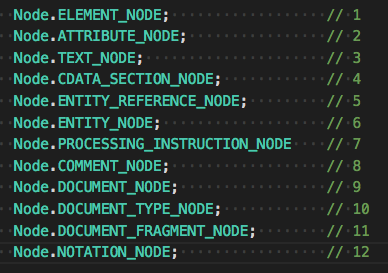
\includegraphics[width=.9\textwidth]{imgs/nodetypes.png}
        \end{center}
     
\end{frame}

\begin{frame}
    \frametitle{Visualizzare ed Elaborare documenti XML}
    \addtocounter{nframe}{1}
    
    %\begin{center}
    %    
\includegraphics[width=.2\textwidth]{../imgs/tei-r.pdf}
    %\end{center}
    %\textit{In parte già disponibili nei moduli TEI di base}

     \begin{block}{Il Modello DOM: principali caratteristiche}
        \begin{itemize}
            \item All nodes in a document have hierarchical relationships to other nodes
            \item Each node has a childNodes property containing a NodeList
        \end{itemize}
     \end{block}

     \begin{block}{Il Modello DOM: principali caratteristiche}

            A NodeList is an array-like object used to store an ordered list of nodes that are accessible by position
       
     \end{block}

\end{frame}

\begin{frame}
    \frametitle{Visualizzare ed Elaborare documenti XML}
    \addtocounter{nframe}{1}
    
    %\begin{center}
    %    
\includegraphics[width=.2\textwidth]{../imgs/tei-r.pdf}
    %\end{center}
    %\textit{In parte già disponibili nei moduli TEI di base}

     \begin{block}{Il Modello DOM: esempio NodeList}
        \texttt{firstChild = someNode.childNodes[0];}
        \\\texttt{secondChild = someNode.childNodes.item(1); }
        \\\texttt{count = someNode.childNodes.length;}
     \end{block}

\end{frame}

\begin{frame}
    \frametitle{Visualizzare ed Elaborare documenti XML}
    \addtocounter{nframe}{1}
    
    \begin{center}
        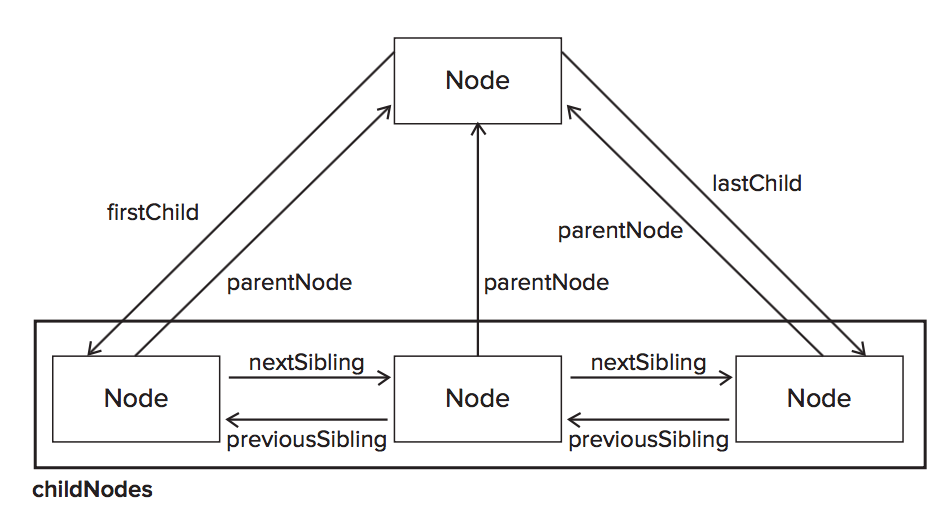
\includegraphics[width=.8\textwidth]{imgs/nodeRelations.png}
    \end{center}
    %\textit{In parte già disponibili nei moduli TEI di base}

\end{frame}

\begin{frame}
    \frametitle{Visualizzare ed Elaborare documenti XML}
    \addtocounter{nframe}{1}
    
    %\begin{center}
    %    
\includegraphics[width=.2\textwidth]{../imgs/tei-r.pdf}
    %\end{center}
    %\textit{In parte già disponibili nei moduli TEI di base}

     \begin{block}{Il Modello DOM: proprietà ownerDocument}
        Tutti i nodi condividono la proprietà \texttt{ownerDocument} che è un collegamento diretto al nodo che rappresenta l'intero documento.
     \end{block}

     \begin{block}{Il Modello DOM: proprietà ownerDocument}
        This property provides a quick way to access the document node without needing to traverse the node hierarchy back up to the top.
     \end{block}

\end{frame}

\begin{frame}
    \frametitle{Visualizzare ed Elaborare documenti XML}
    \addtocounter{nframe}{1}
    
    %\begin{center}
    %    
\includegraphics[width=.2\textwidth]{../imgs/tei-r.pdf}
    %\end{center}
    %\textit{In parte già disponibili nei moduli TEI di base}

     \begin{block}{Il Modello DOM: metodi per la manipolazione}
        Una serie di metodi sono disponibile per la manipolazione dei nodi dell'albero DOM.
     \end{block}

     \begin{block}{Il Modello DOM: metodi per la manipolazione}
        Quattro di questi metodi (sei in totali) lavorano sui figli di uno specifico nodo:
        \\poiché non tutti i tipi di nodi hanno nodi figli questi ultimi metodi possono lanciare degli errori se invocati.
     \end{block}

\end{frame}

\begin{frame}
    \frametitle{Visualizzare ed Elaborare documenti XML}
    \addtocounter{nframe}{1}
    
    %\begin{center}
    %    
\includegraphics[width=.2\textwidth]{../imgs/tei-r.pdf}
    %\end{center}
    %\textit{In parte già disponibili nei moduli TEI di base}

     \textit{Il Modello DOM: metodi per la manipolazione}
       
    \begin{center}
        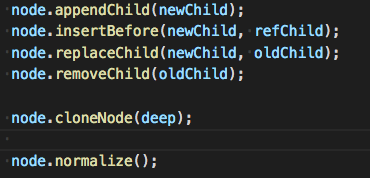
\includegraphics[width=.9\textwidth]{imgs/nodeManipulation.png}
    \end{center}
     
\end{frame}


%% piccolo approfondimento su Document Type - Element Type - Text Type - Attribute Type

\begin{frame}
    \frametitle{Visualizzare ed Elaborare documenti XML}
    \addtocounter{nframe}{1}
    
    %\begin{center}
    %    
\includegraphics[width=.2\textwidth]{../imgs/tei-r.pdf}
    %\end{center}
    %\textit{In parte già disponibili nei moduli TEI di base}

     \begin{block}{Il Modello DOM: Document Type}
        \begin{itemize}
            \item Represents an entire document and is the root node of a hierarchy
            \item The document object is an instance of Document type, which allows for querying and retrieval of nodes in a number of different ways.
        \end{itemize}
     \end{block}

     \begin{block}{Il Modello DOM: Document Type esempio}

            \texttt{xmlRootElement = document.documentElement;}
            \\\texttt{divElement = document.getElementById('divID');}
            \\\texttt{myDivList = document.getElementsByTagName('div');}
       
     \end{block}

\end{frame}

\begin{frame}
    \frametitle{Visualizzare ed Elaborare documenti XML}
    \addtocounter{nframe}{1}
    
    %\begin{center}
    %    
\includegraphics[width=.2\textwidth]{../imgs/tei-r.pdf}
    %\end{center}
    %\textit{In parte già disponibili nei moduli TEI di base}

     \begin{block}{Il Modello DOM: Element Type}
        \begin{itemize}
            \item Rappresenta elementi XML (ma anche HTML) in un documento
            \item Usato per accedere e manipolare  il proprio contenuto e li valore degli attributi 
        \end{itemize}
     \end{block}

     \begin{block}{Il Modello DOM: Element Type esempio}

        \texttt{myDiv.tagName == myDiv.nodeName}
        \\\texttt{if (element.tagName.toLowerCase() == “div”){// istruzioni varie}}
       
     \end{block}

\end{frame}

\begin{frame}
    \frametitle{Visualizzare ed Elaborare documenti XML}
    \addtocounter{nframe}{1}
    
    %\begin{center}
    %    
\includegraphics[width=.2\textwidth]{../imgs/tei-r.pdf}
    %\end{center}
    %\textit{In parte già disponibili nei moduli TEI di base}

     \begin{block}{Il Modello DOM: Attribute Type}
        \begin{itemize}
            \item Technically, attributes are nodes that exist in an element’s attributes property.
            \item Child nodes may be Text or EntityReference in XML.
        \end{itemize}
     \end{block}

     \begin{block}{Il Modello DOM: Attribute Type esempio}

        \texttt{myDiv.getAttribute('lang');}
        \\\texttt{attr = document.createAttribute("rend");} 
        \\\texttt{attr.value = "above";} 
        \\\texttt{element.setAttributeNode(attr);}
       
     \end{block}

\end{frame}

\begin{frame}
    \frametitle{Visualizzare ed Elaborare documenti XML}
    \addtocounter{nframe}{1}
    
    %\begin{center}
    %    
\includegraphics[width=.2\textwidth]{../imgs/tei-r.pdf}
    %\end{center}
    %\textit{In parte già disponibili nei moduli TEI di base}

     \begin{block}{Il Modello DOM: Text Type}
        \begin{itemize}
            \item contain plain text that is interpreted literally and may contain escaped XML characters but no XML code.
            \item very element that may contain content will have al meno one text node when content is present
        \end{itemize}
     \end{block}

     \begin{block}{Il Modello DOM: Text Type esempio}

        \texttt{var textNode = myDiv.firstChild;}
        \\\texttt{var text = textNode.nodeValue;}
        \\\texttt{var newTextNode = document.createTextNode(' testo aggiunto');}
        \\\texttt{myDiv.appendChild(newTextNode);}
        \\\texttt{ myDiv.normalize();}
        \\\texttt{element.firstChild.splitText(5);}
       
     \end{block}

\end{frame}


\begin{frame}
    \frametitle{Visualizzare ed Elaborare documenti XML}
    \addtocounter{nframe}{1}
    
    %\begin{center}
    %    
\includegraphics[width=.2\textwidth]{../imgs/tei-r.pdf}
    %\end{center}
    %\textit{In parte già disponibili nei moduli TEI di base}

     \begin{block}{Modello DOM per la manipolazione di documenti XML}
        DOM Levels 2 and 3 Core is to expand the DOM API to encompass all of the requirements of XML.
     \end{block}

     \begin{block}{Verificare con js se il browser implementa i moduli XML del modello DOM}
        \texttt{document.implementation.hasFeature(“Core”, “2.0”); }
        \\\texttt{document.implementation.hasFeature(“Core”, “3.0”);} 
        \\\texttt{document.implementation.hasFeature(“XML”, “2.0”);}
     \end{block}
     
\end{frame}

\begin{frame}
    \frametitle{Visualizzare ed Elaborare documenti XML}
    \addtocounter{nframe}{1}
    
    %\begin{center}
    %    
\includegraphics[width=.2\textwidth]{../imgs/tei-r.pdf}
    %\end{center}
    %\textit{In parte già disponibili nei moduli TEI di base}

     \begin{block}{Modello DOM verificare lo stato dell'implementazione}
        
        The document .implementation property is an object containing information and functionality tied directly to the browser’s implementation of the DOM
     \end{block}

     \begin{block}{Modello DOM verificare lo stato dell'implementazione}
        It’s very easy to make this method return true for any and all values, but that doesn’t necessarily mean that the implementation conforms to all the specifications it claims to.
     \end{block}
     
\end{frame}


\begin{frame}
    \frametitle{Visualizzare ed Elaborare documenti XML}
    \addtocounter{nframe}{1}
    
    %\begin{center}
    %    
\includegraphics[width=.2\textwidth]{../imgs/tei-r.pdf}
    %\end{center}
    %\textit{In parte già disponibili nei moduli TEI di base}

     \begin{block}{Modello DOM per XML: Level 2 e Level 3}
        \begin{itemize}
            \item  DOM Level 2 Core introduces several new methods related to XML namespaces on various DOM types
            \item DOM Leve 2 permette la creazione di new instances of Document and to enable the creation of DocumentType objects
        \end{itemize}
       
     \end{block}

     
\end{frame}

\begin{frame}
    \frametitle{Visualizzare ed Elaborare documenti XML}
    \addtocounter{nframe}{1}
    
    %\begin{center}
    %    
\includegraphics[width=.2\textwidth]{../imgs/tei-r.pdf}
    %\end{center}
    %\textit{In parte già disponibili nei moduli TEI di base}

     \begin{block}{Modello DOM per XML: Traversals e Range}
        \begin{itemize}
            \item The DOM Level 2 Traversals and Range module specifies different ways to interact with a DOM structure as follows
            \item Oggetti \texttt{NodeIterator} e \texttt{TreeWalker} per eseguire "attraversamenti" \textbf{depth-first} sull'albero DOM.
        \end{itemize}
       
     \end{block}

     \begin{block}{Modello DOM per XML: Traversals e Range}
        \begin{itemize}
            \item Ranges are a way to select specific portions of a DOM structure to augment it in some fashion.
            \item can be used to remove portions of a document while retaining a well-formed document structure or for cloning portions of a document.
        \end{itemize}
       
     \end{block}

     
\end{frame}


\begin{frame}
    \frametitle{Visualizzare ed Elaborare documenti XML}
    \addtocounter{nframe}{1}
    
    %\begin{center}
    %    
\includegraphics[width=.2\textwidth]{../imgs/tei-r.pdf}
    %\end{center}
    %\textit{In parte già disponibili nei moduli TEI di base}

     \begin{block}{Modello DOM per XML}
        \begin{itemize}
            \item DOM Level 2 introduce il concetto di creazione dinamica di documenti XML
            \item DOM Level 3 introduce meccanismi di parsing e di serializzazione XML.
        \end{itemize}
        
     \end{block}

     \begin{block}{modello DOM per XML: creazione di documenti}
       
       % \\\texttt{document.implementation.hasFeature(“Core”, “3.0”);} 
       % vedere capitolo 12
       \texttt{xmlDom = document.implementation.createDocument(}
        \\\texttt{   namespaceUri, root, doctype);;} 
        \texttt{teiDom = document.implementation.createDocument(}
        \\\texttt{   'http://www.tei-c.org/ns/1.0', 'tei:TEI', TEIDoctype);;} 
       
     \end{block}
     
\end{frame}


\begin{frame}
    \frametitle{Visualizzare ed Elaborare documenti XML}
    \addtocounter{nframe}{1}
    
    %\begin{center}
    %    
\includegraphics[width=.2\textwidth]{../imgs/tei-r.pdf}
    %\end{center}
    %\textit{In parte già disponibili nei moduli TEI di base}

     \begin{block}{Modello DOM per XML}
        \begin{itemize}
            \item Una volta creato il documento è possibile sfruttare tutte le features che ci mette a disposizione il modello DOM.
            \item Nuovi nodi possono essere aggiunti al documento e manipolati a piacimento.
        \end{itemize}
        
     \end{block}

     \begin{block}{modello DOM per XML: creazione di documenti}
       
       % \\\texttt{document.implementation.hasFeature(“Core”, “3.0”);} 
       % vedere capitolo 12
       \texttt{teiHeaderElem = teiDom.createElement('teiHeader'); }
       \\\texttt{teiDom.documentElement.appendChild(teiHeaderElem);}
       
     \end{block}
     
\end{frame}


\begin{frame}
    \frametitle{Visualizzare ed Elaborare documenti XML}
    \addtocounter{nframe}{1}
    
    %\begin{center}
    %    
\includegraphics[width=.2\textwidth]{../imgs/tei-r.pdf}
    %\end{center}
    %\textit{In parte già disponibili nei moduli TEI di base}

     \begin{block}{Modello DOM per XML}
        \begin{itemize}
            \item  It is much more likely that an XML document needs to be parsed into a DOM structure or vice versa
            \item Esiste un oggetto  \texttt{DOMParser} che può "parsare" stringhe di testo che rappresentato documenti XML \textbf{well-formed}
        \end{itemize}
        
     \end{block}

     \begin{block}{modello DOM per XML: creazione di documenti}
       
       % \\\texttt{document.implementation.hasFeature(“Core”, “3.0”);} 
       % vedere capitolo 12
        \texttt{parser = new DOMParser();}
        \\\texttt{teiDoc = parser.parseFromString(“<TEI><teiHeader/></TEI>”, “text/xml”);}
        \\\texttt{textElement = teiDoc.createElement("text");}
        \\\texttt{teiDoc.documentElement.appendChild(textElement);}
        
     \end{block}
     
\end{frame}


\begin{frame}
    \frametitle{Visualizzare ed Elaborare documenti XML}
    \addtocounter{nframe}{1}
    
    %\begin{center}
    %    
\includegraphics[width=.2\textwidth]{../imgs/tei-r.pdf}
    %\end{center}
    %\textit{In parte già disponibili nei moduli TEI di base}

     \begin{block}{Modello DOM per XML}
        \begin{itemize}
            \item Esiste anche l'oggetto duale di \texttt{DOMParser}. Questo è l'oggetto \texttt{XMLSerializer}.
            \item  per ottenere una stringa che rappresenti il documento XML bisogna creare una istanza di \texttt{XMLSerializer} e passare al metodo \texttt{serializeToString()} il documento DOM.
        \end{itemize}
        
     \end{block}

     \begin{block}{modello DOM per XML: serializzazione di documenti}
       
       % \\\texttt{document.implementation.hasFeature(“Core”, “3.0”);} 
       % vedere capitolo 12
        \texttt{serializer = new XMLSerializer();}
        \\\texttt{xml = serializer.serializeToString(xmldom);}
        
     \end{block}
     
\end{frame}

\begin{frame}
    \frametitle{Visualizzare ed Elaborare documenti XML}
    \addtocounter{nframe}{1}
    
    %\begin{center}
    %    
\includegraphics[width=.2\textwidth]{../imgs/tei-r.pdf}
    %\end{center}
    %\textit{In parte già disponibili nei moduli TEI di base}

     \begin{block}{Modello DOM per XML}
        \begin{itemize}
            \item Non è disponibile un metodo diretto per caricare XML da server o da file in locale. 
            \item Solo Internet Explorer ha sviluppato nativamente una funzionalità del genere sul DOM \texttt{(xmldom.load("example.xml")}).
            \item E' generalmente accettato utilizzare l'oggetto XMLHttpRequest per caricare file da percorsi esterni (remoti oppure locali).
        \end{itemize}
        
     \end{block}

     
\end{frame}

\begin{frame}
    \frametitle{Visualizzare ed Elaborare documenti XML}
    \addtocounter{nframe}{1}
    
    %\begin{center}
    %    
\includegraphics[width=.2\textwidth]{../imgs/tei-r.pdf}
    %\end{center}
    %\textit{In parte già disponibili nei moduli TEI di base}

    \textit{Il più delle volte è meglio utilizzare chiamate asincrone e non sincrone per caricare risorse esterne.}

     \begin{block}{modello DOM per XML: caricamento di documenti}
       
       % \\\texttt{document.implementation.hasFeature(“Core”, “3.0”);} 
       % vedere capitolo 12
        \texttt{xhr = new XMLHttpRequest();}
        \\\texttt{xhr.open(“get”, “example.txt”, false);} 
        \\\texttt{xhr.send(null);}
        \\\texttt{if ((xhr.status >= 200 && xhr.status < 300) || xhr.status == 304)}
        \\\texttt{{ text = xhr.responseText); } else { ... }}
        
     \end{block}
     
\end{frame}


     
\end{frame}

\begin{frame}
    \frametitle{Visualizzare ed Elaborare documenti XML}
    \addtocounter{nframe}{1}
    
    %\begin{center}
    %    
\includegraphics[width=.2\textwidth]{../imgs/tei-r.pdf}
    %\end{center}
    %\textit{In parte già disponibili nei moduli TEI di base}

    \begin{block}{modello DOM per XML: Xpath}
        An API for XPath wasn’t part of a specification until DOM Level 3, which introduced the DOM Level 3 XPath recommendation
    \end{block}

     \begin{block}{modello DOM per XML: Xpath}
       
       % \\\texttt{document.implementation.hasFeature(“Core”, “3.0”);} 
       % vedere capitolo 12
       \texttt{var supportsXPath = document.implementation.hasFeature(“XPath”, “3.0”);}
        
        
     \end{block}
     
\end{frame}

\begin{frame}
    \frametitle{Visualizzare ed Elaborare documenti XML}
    \addtocounter{nframe}{1}
    
    %\begin{center}
    %    
\includegraphics[width=.2\textwidth]{../imgs/tei-r.pdf}
    %\end{center}
    %\textit{In parte già disponibili nei moduli TEI di base}

    \begin{block}{modello DOM per XML: Xpath}
        \begin{itemize}
            \item Oggetto di tipo \texttt{XPathEvaluator} (used to evaluate XPath expressions)
            \item Oggetto di tipo \texttt{XPathResult} (impiegato per gestire il tipo di risultato ottenuto da una operazione di selezione xpath)
        \end{itemize}
       
    \end{block}

     \begin{block}{modello DOM per XML: Xpath}
       
       % \\\texttt{document.implementation.hasFeature(“Core”, “3.0”);} 
       % vedere capitolo 12
       \texttt{result = xmldom.evaluate(“employee/name”, xmldom.documentElement, null, XPathResult.ORDERED_NODE_ITERATOR_TYPE, null);}
       \\\texttt{evaluator.evaluate(expression, contextNode, resolver, type, result)}
        
        
     \end{block}
     
\end{frame}


\begin{frame}
    \frametitle{Visualizzare ed Elaborare documenti XML}
    \addtocounter{nframe}{1}
    
    \textbf{XPathResult ha 10 tipi diversi di possibili valori}

    \begin{center}
        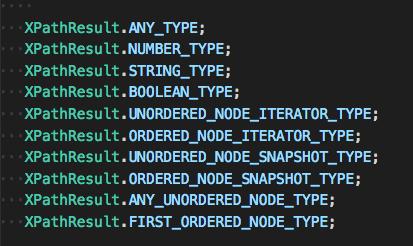
\includegraphics[width=.9\textwidth]{imgs/xpathResult.png}
    \end{center}

\end{frame}

\begin{frame}
    \frametitle{Visualizzare ed Elaborare documenti XML}
    \addtocounter{nframe}{1}
    
    %\begin{center}
    %    
\includegraphics[width=.2\textwidth]{../imgs/tei-r.pdf}
    %\end{center}
    %\textit{In parte già disponibili nei moduli TEI di base}

    \begin{block}{modello DOM per XML: Xpath Esempio}
        \texttt{result = xmldom.evaluate(}
         \\\texttt{ 'text/back', xmlTEI.documentElement, }
         \\\texttt{ null, XPathResult.BOOLEAN_TYPE, null);}
    \end{block}

     \begin{block}{modello DOM per XML: Xpath Esempio}
        \texttt{result = xmldom.evaluate(}
        \\\texttt{  'count(text/body/div)', xmldom.documentElement,} 
        \\\texttt{  null, XPathResult.NUMBER_TYPE, null);}
     \end{block}
     
\end{frame}

\begin{frame}
    \frametitle{Visualizzare ed Elaborare documenti XML}
    \addtocounter{nframe}{1}
    
    %\begin{center}
    %    
\includegraphics[width=.2\textwidth]{../imgs/tei-r.pdf}
    %\end{center}
    %\textit{In parte già disponibili nei moduli TEI di base}

    \begin{block}{modello DOM per XML: Namespace support}
        \begin{itemize}
            \item Spesso i documenti XML fanno uso di namespace per qualificate il corretto vocabolario impiegato.
            \item In questa ciscostanza \texttt{XPathEvaluator} deve essere opportunamente impostato.
            \item Nel documenti TEI-XML tutti gli elementi sono parte del namespace \texttt{http://www.tei-c.org/ns/1.0}
        \end{itemize}
        
    \end{block}
     
\end{frame}


\begin{frame}
    \frametitle{Visualizzare ed Elaborare documenti XML}
    \addtocounter{nframe}{1}
    
    %\begin{center}
    %    
\includegraphics[width=.2\textwidth]{../imgs/tei-r.pdf}
    %\end{center}
    %\textit{In parte già disponibili nei moduli TEI di base}

    \begin{block}{modello DOM per XML: Namespace support}
        \begin{itemize}
            \item Un modo per gestire il namespace è attraverso la creazione di un oggetto \texttt{XPathNSResolver}
            \item Invocando il metodo \texttt{createNSResolver()} del documento.
            \item Struttando una funzione che dato un prefisso restituisce l'URI del namespace. (\texttt{lookupNamespaceURI})
        \end{itemize}
    \end{block}

    \begin{block}{modello DOM per XML: Namespace support example}
        \texttt{nsresolver = xmldom.createNSResolver(xmldom.documentElement);} 
        \\\texttt{result = xmldom.evaluate(} \\\texttt{"/tei:TEI/tei:text/tei:front/tei:titlePage/tei:docImprint/tei:publisher",} \\\texttt{xmldom.documentElement, nsresolver, XPathResult.ORDERED_NODE_SNAPSHOT_TYPE, null);}
    \end{block}
     
\end{frame}

\begin{frame}
    \frametitle{Visualizzare ed Elaborare documenti XML}
    \addtocounter{nframe}{1}
    
    %\begin{center}
    %    
\includegraphics[width=.2\textwidth]{../imgs/tei-r.pdf}
    %\end{center}
    %\textit{In parte già disponibili nei moduli TEI di base}

    \begin{block}{modello DOM per XML: XSLT support}
        \begin{itemize}
            \item Esiste un oggetto che può essere usato per elaborare fogli di stile XSLT in javascript: \texttt{XSLTProcessor}.
            \item Il promo passo è caricare due documenti DOM: un XML di base, e l'altro XSLT.
        \end{itemize}
    \end{block}

    \begin{block}{modello DOM per XML: XSLT support example}
         \texttt{processor = new XSLTProcessor()} 
         \\\texttt{processor.importStylesheet(xsltdom);}
         \\\text{result = processor.transformToDocument(xmldom);}
    \end{block}
     
\end{frame}

\begin{frame}
    \frametitle{Visualizzare ed Elaborare documenti XML}
    \addtocounter{nframe}{1}
    
    %\begin{center}
    %    
\includegraphics[width=.2\textwidth]{../imgs/tei-r.pdf}
    %\end{center}
    %\textit{In parte già disponibili nei moduli TEI di base}

    \begin{block}{modello DOM per XML: XSLT support}
        \begin{itemize}
            \item Accanto al metodo \texttt{transformToDocument()} esiste anche il metodo  \testtt{transformToFragment()}. 
            \item La ragione per l'utilizzo di tale metodo è per coprire eventuali casi in cui il risultato della trasformazione vuole essere aggiunta ad un terzo documento DOM.
            \item Tra gli argomenti, infatti, deve essere inserito anche il documento destinatario finale per ovvi controlli di consistenza.
        \end{itemize}
    \end{block}

    \begin{block}{modello DOM per XML: XSLT support example}
        \testtt{fragment = processor.transformToFragment(xmldom, document); }
        \\\texttt{div = document.getElementById(“divResult”); }
        \\\texttt{div.appendChild(fragment);}
    \end{block}
     
\end{frame}

\begin{frame}
    \frametitle{Visualizzare ed Elaborare documenti XML}
    \addtocounter{nframe}{1}
    
    %\begin{center}
    %    
\includegraphics[width=.2\textwidth]{../imgs/tei-r.pdf}
    %\end{center}
    %\textit{In parte già disponibili nei moduli TEI di base}

    \begin{block}{modello DOM per XML: XSLT support}
        L'oggetto XSLTProcessor permette di gestire e indicare parametri XSLT
    \end{block}

    \begin{block}{modello DOM per XML: XSLT support example}
         \texttt{processor = new XSLTProcessor();}
         \\\texttt{processor.importStylesheet(xsltdom);} 
         \\\texttt{processor.setParameter(null, "message", "contenuto del messaggio");} 
         \\\texttt{result = processor.transformToDocument(xmldom);}
    \end{block}
     
\end{frame}

\begin{frame}
    \frametitle{Visualizzare ed Elaborare documenti XML}
    \addtocounter{nframe}{1}
    
    %\begin{center}
    %    
\includegraphics[width=.2\textwidth]{../imgs/tei-r.pdf}
    %\end{center}
    %\textit{In parte già disponibili nei moduli TEI di base}

    \begin{block}{modello DOM per XML: XSLT support}
        Le istanze dell'oggetto \texttt{XSLTProcessor} possono essere riusate per più trasformazioni e con diversi fogli di stile (Efficienza computazionale).
    \end{block}

    \begin{block}{modello DOM per XML: XSLT support example}
        \texttt{processor.importStylesheet(xsltdom); }
        \\\texttt{//do some transformations }
        \\\texttt{processor.reset(); }
        \\\texttt{processor.importStylesheet(xsltdom2); }
    \end{block}
     
\end{frame}

\begin{frame}
    \frametitle{Visualizzare ed Elaborare documenti XML}
    \addtocounter{nframe}{1}
    
    %\begin{center}
    %    
\includegraphics[width=.2\textwidth]{../imgs/tei-r.pdf}
    %\end{center}
    %\textit{In parte già disponibili nei moduli TEI di base}

    \begin{block}{modello DOM per XML: concludendo..}
       la tecnologia XML è ad oggi ben supportato nei vari browser, anche se alcune implementazioni differiscono in termini di copertura dello standard e di aderenza ad esso. Esistono comunque tecnologie per avere un supporto cross-browser per le più comuni funzionalità.
    \end{block}
     
\end{frame}



